\begin{lemma}[Sum of Gamma random variables]
    \label{stats/4/gamma}
Suppose that $X_i \sim \Gamma(k, \theta), i = 1, \dots, n$. Then $T = \sum_{i=1}^{n} X_i \sim \Gamma(nk, \theta)$.
\end{lemma}
\begin{definition}[Laplace transform]
    Laplace transform is an integral transform that converts a real function of a real variable $t$ to a function of a complex variable $s$. The laplace transform of a function $f(t)$ evaluated at $s$ is defined by
    \begin{align}
    F(s) = \int_0^{\infty} f(t) e^{-st} dt
    \end{align}
    \end{definition}
    \begin{lemma}
    \label{stats/6/lemma_laplace_transform}
    If the laplace transform of a function $f(t)$ at $s$ is $0$ for all $s>0$, then the function $f(t) = 0$ almost everywhere in $(0, \infty)$.
    \end{lemma}
\begin{definition}[Complete Statistic]
The statistic $T$ is said to be complete for the distribution of $X$ if, for every measurable function $g$, if
\begin{align}
E(g(T)) = 0 \; \forall \; \theta \Rightarrow \pr{g(T)=0} = 1 
\end{align}
\end{definition}
\begin{definition}[Sufficient Statistic]
A statistic $t = T(X)$ is sufficient for underlying parameter $\theta$ precisely if the conditional probability distribution of the data $X$, given the statistic $t = T(X)$, does not depend on the parameter $\theta$. 
\end{definition}
\begin{theorem}[Fischer-Neymann Factorisation theorem]
If the probability density function is $f_\theta (x)$, then $T$ is sufficient for $\theta$ if and only if nonnegative functions $g$ and $h$ can be found such that
\begin{align}
f_\theta (x) = h(x)g_\theta(T(x))
\end{align}
\end{theorem}
\begin{lemma} \label{stats/6/lemma_sufficient_complete}
\begin{align}
T = \sum_{i=1}^{n} X_i
\end{align}
is a complete and sufficient statistic. 
\end{lemma}
\begin{proof}
\begin{enumerate}
\item \textit{(Sufficiency)}
\begin{align}
f_{X}(x_1, x_2, \ldots x_n) &= \prod_{i=1}^{n}f_{X_i}(x_i)\\
&= \prod_{i=1}^{n} \dfrac{1}{\theta} \exp\brak{-\dfrac{x_i}{\theta}} \\
&= 1 \cdot \dfrac{1}{\theta^n} \exp\brak{-\dfrac{T}{\theta}}\\
&= h(X) \cdot g(T, \theta) 
\end{align}
with 
\begin{align}
g(T, \theta) &= \dfrac{1}{\theta^n} \exp\brak{-\dfrac{T}{\theta}}\\
h(X) &= 1
\end{align}
Therefore, $T$ is a sufficient statistic.
\item \textit{(Completeness)}
From Lemma     \ref{stats/4/gamma}, $X_i \sim \Gamma \brak{1, \frac{1}{\theta}} \implies  T = \sum_{i=1}^n X_i \sim \Gamma \brak{n, \frac{1}{\theta}}$. 
\begin{align}
\therefore E(g(T)) &= 
\int_0 ^{\infty} g(t) \dfrac{t^{n-1} e^{-\frac{t}{\theta}}}{\theta^n(n-1)!} dt\\ 
&= \frac{1}{\theta^n (n-1)!} \int_0 ^{\infty} g(t) t^{n-1} e^{-\frac{t}{\theta}} dt\\ 
&= \frac{1}{\theta^n (n-1)!} F \brak{\frac{1}{\theta}}
%&= 0 \text{ for all } \theta > 0.
\end{align}
where, 
\begin{align}
f(t) &= t^{n-1}g(t) \xrightleftharpoons[]{\mathcal{L}} F \brak{\frac{1}{\theta}}
% &= \text{Laplace Transform of} f(t) \text{ at } \theta
\end{align}
is the Laplace transform relationship.
Then
\begin{align}
E\brak{g(T)}=0 \forall \theta > 0 \implies F \brak{\frac{1}{\theta}} = 0 \forall  \theta > 0
\label{stats/6/eqn}
\\ \implies 
f(t)=0 \text{ a.e } (0, \infty)\\
\text{or, }g(t)=0 \text{ a.e }(0, \infty)\\
\implies \pr{g(t)=0} = 1
\end{align}
from Lemma     \ref{stats/6/lemma_laplace_transform}.  
$\therefore T$ is a complete statistic.
\end{enumerate}
\end{proof}
\begin{theorem}[Lehmann–Scheffé theorem]
If $T$ is a complete sufficient statistic for $\theta$ and 
\begin{align}
\label{eqn 2.0.1}
E(g(T)) = \tau(\theta)
\end{align}
then $g(T)$ is the uniformly minimum-variance unbiased estimator (UMVUE) of $\tau(\theta)$.
\end{theorem}
%
\begin{proposition} \label{stats/6/prop_3.1}
$E(X_{(1)}|T)$ is the uniformly minimum-variance unbiased estimator (UMVUE) of $E(X_{(1)})$
\end{proposition}
\begin{proof}
By the law of total expectation, 
\begin{align}
\label{stats/6/eqn 2.0.3}
E\brak{E(X_{(1)} | T )} = E(X_{(1)})
\end{align}
We know that $T = \sum_{i=1}^n X_i$ is a complete and sufficient statistic by Lemma \ref{stats/6/lemma_sufficient_complete}. By Lehmann–Scheffé theorem, with
\begin{align}
\theta &= X_{(1)},\\ 
\tau(x) &= E(x),\\
g(T) &= E(X_{(1)} | T).
\end{align}
it follows from \eqref{stats/6/eqn 2.0.3} that $E(X_{(1)} | T)$ is the UMVUE of $E(X_{(1)})$.
\end{proof}
\begin{proposition} \label{stats/6/prop_3.2}
$\frac{T}{n^2}$ is uniformly minimum-variance unbiased estimator (UMVUE) of $E(X_{(1)})$
\end{proposition}
\begin{proof}
\begin{enumerate}
\item Let's find the probability distribution function and the expectation value of $X_{(1)}$ : 
\begin{align}
\pr{X_{(1)} > x} &= \pr{X_1 > x}\ldots \pr{X_n > x}\\
&= (1-F_{X_{1}}(x))\ldots(1-F_{X_{n}}(x))\\
&= (1-F_{X_{1}}(x))^n \\
&= \exp\brak{-\frac{nx}{\theta}}\\
F_{X_{(1)}}(x) &= 1 - \exp\brak{-\frac{nx}{\theta}}\\
f_{X_{(1)}}(x) &= \frac{n}{\theta} \exp\brak{-\frac{nx}{\theta}}
\end{align}
Therefore, $X_{(1)}$ follows an exponential distribution with mean $\dfrac{\theta}{n}$.
\begin{align}
E(X_{(1)}) = \frac{\theta}{n}
\end{align}
\item $\frac{T}{n^2}$ is uniformly minimum-variance unbiased estimator (UMVUE) of $E(X_{(1)})$, since $E\brak{\frac{T}{n^2}} = E(X_{(1)})$ : \\
Note that,
\begin{align}
E\brak{\frac{T}{n^2}} &= E\brak{\frac{\sum_{i=1}^n X_i}{n^2}}\\
&= \frac{E(\sum_{i=1}^n X_i)}{n^2}\\
&= \sum_{i=1}^n \frac{E(X_i)}{n^2}\\
&= \sum_{i=1}^n \frac{\theta}{n^2}\\
&= \frac{\theta}{n}\\
&= E(X_{(1)})
\end{align}
\end{enumerate}
Therefore, by Lehmann–Scheffé theorem, with
\begin{align}
\theta &= X_{(1)},\\
\tau(x) &= E(x),\\
g(T) &= \frac{T}{n^2},
\end{align}
it follows that $\dfrac{T}{n^2}$ is UMVUE of $E(X_{(1)})$.\\
\end{proof}
Since there exists a unique UMVUE for $E(X_{(1)})$, it follows from Proposition \ref{stats/6/prop_3.1} and Proposition \ref{stats/6/prop_3.2} that 
\begin{align}
E(X_{(1)} | T) = \frac{T}{n^2} 
\end{align}
Hence, option A is correct.
\begin{figure}[!hbt]
    \centering
	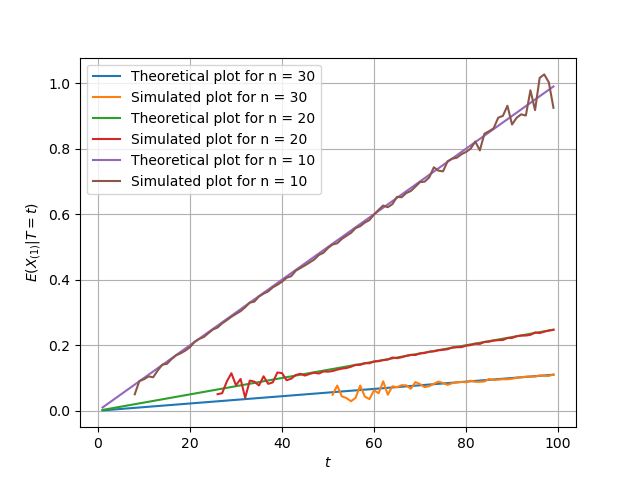
\includegraphics[width=\columnwidth]{stats/solutions/6/Figures/Figure_1.png}
    \caption{Theory vs Simulated plot of $E(X_{(1)} |T)$}
    \label{CDF_Y}
\end{figure}
